

\documentclass[]{article}
\usepackage{graphicx}
\DeclareGraphicsExtensions{.pdf,.png,.jpg}
\usepackage{setspace}
\usepackage{amsmath}
\usepackage{graphicx}
\usepackage[english]{babel}
\usepackage[numbers]{natbib}
\usepackage{url}
\usepackage{ulem} % when using ulem package, must change \emph to \it for italics.
\usepackage{hyperref}
\usepackage{amssymb,tabu}
\usepackage{wrapfig}
\usepackage{lscape}
\usepackage{rotating}
\usepackage{epstopdf}
%\usepackage{hanging}

%TODO: another case with bad data 
%more specific regression interpretation 
%

%opening
\title{The Lieberson Robustness Assessment for Qualitative Comparative Analysis}
\author{Ben Gibson and Burrel Vann Jr}

\begin{document}
\doublespace
\maketitle

\begin{abstract}

Qualitative Comparative Analysis (QCA) has been increasingly used in recent years due to its purported construction of a middle path between case-oriented and variable-oriented methods. Despite it's popularity, the method has been criticized for not distinguishing random from real patterns in data, rendering its usefulness questionable. Stanley Lieberson (), in illustrating this criticism, suggests a straightforward technique to test whether QCA will return a configuration when given random data. We adapt this technique to determine the probability of any given QCA result is due to random chance, which can be used as a robustness assessment for QCA with an interpretation similar to a p-value. Using repeated applications of QCA to randomly-generated data, we first show that generally, the tendency for QCA to return spurious results is greatly attenuated by using reasonable consistency score and configurational n thresholds; however, this varies greatly according to the basic structure of the data, suggesting the need for further robustness assessments. Second, we apply a case-by-case application of this technique to data predicting the occurrence of Tea Party rallies in Florida. This method, which we coin the Lieberson Robustness Assessment for QCA (LaQCA), can provide researchers with case-by-case recommendations for consistency score and configurational n thresholds, while taking into account the structure of the data.

% [Ben] are you calling it laQCA or ltQCA?

\end{abstract}

\section{Introduction}

%Goals: explain how QCA use has expanded 

Qualitative Comparative Analysis (QCA) was introduced in Charles Ragin's 1987 book The Comparative Methods as a "middle-path" technique between quantitative and qualitative analysis. Ragin and others have since published many works on practical applications and extensions of the method, including the use of `fuzzy-sets,' the development of software, and many substantive applications (Caramani 2008; Ragin 2008; Rihoux and Ragin 2009; Schneider and Wagemann 2007, citation on R software). Though originally conceived has a method to analyze middle-sized samples, some herald its interpretive qualities above even regression analysis.

%Goals: explain the benefits of QCA specifically

%Goals: Explain criticisms of the method. Talk about how distinguishing from randomness is a key element of any method (and explain Lieberson's criticism along the way). Talk about recommendations for consistency thresholds are often not based upon real data. 

Despite recent popularity, QCA is not without its detractors. Some have questioned its usefulness, specifically its ability to filter random patterns, a serious problem with any method (). Stanley Lieberson is one such critic (). Lieberson suggested that an application of QCA using random data would often lead to spurious configurations returned. Though many robustness assessments have been undertaken by scholars that assess the effect of user choice on the end results of a QCA analysis, a principled test of QCA against \emph{totally} random data has not been undertaken. 

%Also, add a few sentences about why we care.  (You can mention that this will be further explored in the subsequent section.) 

A principled test of the assessment Lieberson described would be useful in two ways. First, to assess generally the ability of QCA, with reasonable applications of existing robustness parameters (i.e. configurational n and consistency score thresholds) to filter random patterns. Second, with some adjustments, software that assesses the probability of returning random configurations according to unique features of any data set would be useful as a case-by-case robustness assessment for QCA, which currently does not exist. The interpretation of such an assessment would be the probability of returning a random configuration using the data and robustness thresholds selected by the user. This assessment would inform user choice in the use of consistency score and configurational n threshold.

%Introduce the Method

Here, I introduce a method to assess the probability that QCA returns a random result. I systematically apply QCA to thousands of random data sets, incrementally changing elements of the data structure -- sample size and the distribution of variables in the data set -- as well as elements under the control of the researcher -- consistency threshold, configurational n threshold and 'complex' versus 'parsimonious' solutions. I then use logistic regression to determine which of these elements affects the probability of returning a 'random configuration,' or a result returned from random data. 

Importantly, I also describe a related method, to be used on a case-by-case basis, of evaluating any QCA result. This operates by generating many random data sets of the same data structure used in an application of QCA (i.e. based upon the sample size and variable distributions) and applying QCA repeatedly at the parameters under control of the researcher (i.e consistency score thresholds, configurational n, and parsimonious vs. complex solutions). The result is the probability that a QCA configuration returned is due to random chance, based upon random data of similar size and distribution. I hope that this method will provide straightforward recommendations for researchers who look for unarbitrarily drawn parameters of choice. 


\section{QCA's Randomness Problem}

%Lieberson's criticisms 

Lieberson's chief criticism of QCA is that "QCA is less prepared to allow for chance and probabilistic processes" than other methods and that "procedures do not rule out the possibility that the observations are all a random matter" (13). He imagines a test of this assertion: apply QCA to a collected data set versus a set where values were randomly reassigned, keeping the marginal distributions intact. If QCA returns a configuration in both cases, it has a serious problem with being able to distinguish real patterns from random ones. 

In a rebuttal, Ragin and Rihoux (2004) argue that such a test would show that random patterns would be filtered out by probabilistic procedures -- namely, the use of a high consistency threshold (i.e. the proportion of cases that are explained given a configuration) and a reasonable configuration n threshold (i.e. the number of cases that have a certain of causal conditions). The utility of these procedures to distinguish a random data set from a collected one is an empirical question, however,. 

The rebuttal also claims that the test would be irrelevant, because the researcher would observe several contradictory cases in the randomly-drawn data set, and would be able to spot them in the execution of QCA. We cannot escape, however, that certain properties of data sets outside of researcher control -- namely the marginal distribution of causal conditions included in the analysis -- greatly increase the chance that spurious configurations will be returned when applied to a random data set. 

For example, imagine a QCA analysis had three causal conditions and an outcome, each variable having a .9 probability of being "1." As a baseline, we know that cases have a $.9^4 = 0.6561$ probability of all variables being "1." To deal with this, QCA has thresholds to filter out totally random results like this. For example, a consistency threshold of .7 (a very low threshold) would ostensibly prevent such a random result from occurring. However, given the relatively few cases used in QCA, such a result would not easily be filtered using less than 100 or so cases. Repeated random selection of cases into these categories would actually be rather unstable, with wide intervals surrounding the .6561 figure. 



%Figure 1 shows a repeated simulation of 30 cases with these exact marginal probabilities -- each causal condition having a .9 probability of being positive and the outcome having a .9 probability of being negative.

%PLOT: differential effect of consistency score threshold upon randomness given 

We can thus see that depending upon the distribution of variables in an observed QCA data set, there is a large difference in the baseline chance of a random result depending upon the marginal distribution of variable in the data set. (We test this hypothesis below.)


%TODO: Do this plot

%Summary 

This paper first tests which analysis thresholds are important for filtering out random configurations; we then test whether reasonable thresholds of analysis can be used to filter out most random configurations. We then apply a general method for testing whether a QCA result is robust to randomness given both the data structure and the thresholds chosen by the researcher. 


\section{Is QCA Robust to Randomness?}

%Researcher choice in QCA and the need for principled recommendations

The randomness problem with QCA is well-documented (cite) and there are thresholds available to set prior to the analysis to reduce random configurations from being returned. The \emph{consistency threshold} restricts the analysis to only considering configurational categories that have a certain proportion of cases that all agree in the direction of the dependent variable. The \emph{configurational n threshold} restricts the analysis to only consider those configurational categories that have a certain number of cases within them. For example, we can choose to only include those combinations of causal conditions that have four or more cases that share all of the same causal condition states. The choice of using all [Ben: explain the difference between using parsimonious versus complex solutions] is another way to attempt to filter out random configurations.

Though these are attempts to introduce probabilistic checks for QCA configurations, their use is often flexible, and general recommendations for which thresholds are hard to determine without principled testing of their usefulness. This section assesses the relative importance of each probabilistic check for filtering out random configurations from being returned by QCA. 


\subsection{Assessing the Robustness of QCA}

We employ a straightforward assessment of QCA using simulations. At each iteration, we first simulate a random data set. Next, we apply QCA to the random data set, and record whether QCA returned result at all from random data. If we discover that a result is returned, we know that QCA is returning a spurious result. We systematically vary several variables to determine which elements of data structure (marginal distribution of variables, number of causal conditions included in the model, and sample size) and features of researcher choice (consistency threshold and configurational n threshold) affect the probability of a spurious result.  %Below, we describe the factors we altered to determine which facets of the data and analysis most affect the probability that a random configuration is returned from QCA.

In these simulations, each causal condition is a dummy variable with a marginal distribution varying between .1 to .9 probability of being "1." Though variables vary between iterations, all variables have the same marginal distribution within each iteration. The number of causal conditions vary from one to six. The sample size varies from 10 to 100. Between iterations, we systematically vary the configurational n threshold from one to six. We vary the consistency threshold from .5 to 1.

We employ logistic regression on the results, with the dependent variable being a 0-1 outcome of returning a configuration from random data. The independent variables are the factors listed in Table 1. The primary question here is, which factors, when altered, independently decrease the probability of returning a random configuration?

Secondly, we assess whether researcher choice differentially affects the probability of a result given the structure of the data. For example, does a high consistency score threshold filter spuriousness across all sample sizes? Does a high configurational n threshold filter spuriousness given all marginal probabilities of causal conditions? This is tested using interaction effects between variables measuring researcher choice and variables measuring data structure. If interaction effects are substantial, it suggests that additional assessments that take into account data structure need to applied to QCA to ensure robustness.


\subsection{Results: the Effects of Data Structure and Researcher Choice on Spuriousness}

Table 1 shows the results of the logistic regression model predicting whether QCA returned a spurious result from simulated random data. The largest effect is the effect for the distribution of variables -- the marginal distribution for all variables in the data set. An increase in all marginal distributions from 0 to 1 increased the logged odds of a spurious result by 4.8 (about 170 times the odds). Increasing the number of variables also increases the probability of a spurious result. Interestingly, increasing the sample size also increases the probability of a spurious result. This is in contrast to other mean-based approaches which typically become more robust as sample size increases.



% latex table generated in R 3.0.2 by xtable 1.7-3 package
\begin{table}[ht]
\caption {\textbf{Logistic Regression Predicting the Probability of Returning a Spurious Configuration in csQCA}} \label{tab:title}
%\centering
\begin{tabular}{lrr}
  \hline
 Variable & Model 1 & Model 2 \\ 
  \hline
  Intercept & -1.23 (0.02)$ ^{***}$ & 2.62 (0.12)$ ^{***}$    \\ 
  Cons. Threshold & -2.54 (0.02)$ ^{***}$ & -9.16 (0.15)$ ^{***}$ \\ 
  Conf. N Threshold & -0.55 (0.00)$ ^{***}$ & -0.37 (0.01)$ ^{***}$  \\ 
  Sample Size & 0.01 (0.00)$ ^{***}$ & 0.02 (0.00)$ ^{***}$  \\ 
  N. Vars & 0.19 (0.00)$ ^{***}$ & -0.01 (0.02) \\ 
  Distribution & 4.80 (0.01)$ ^{***}$ & -0.53 (0.11)$ ^{***}$  \\ 
  Cons. Threshold*N. Vars & & 0.92 (0.02)$ ^{***}$   \\ 
  Cons. Threshold*Distribution & & 5.80 (0.13)$ ^{***}$  \\ 
  Conf. N Threshold*N. Vars & & -0.15 (0.00)$ ^{***}$  \\ 
  Conf. N Threshold*Distribution & & 0.45 (0.01)$ ^{***}$  \\ 
  Residual Deviance &  759400 & 239819 \\
   \hline
 \multicolumn{2}{l}{\footnotesize{Null Deviance: 1121663}}\\
 \multicolumn{1}{l}{\footnotesize{$^{*}p < .05$, $ ^{**}p < .01 $,  $ ^{***}p < .001 $}}\\

\end{tabular}
\end{table}



\begin{sidewaysfigure}[htb!]
\label{diagram}
	%\begin{center}
	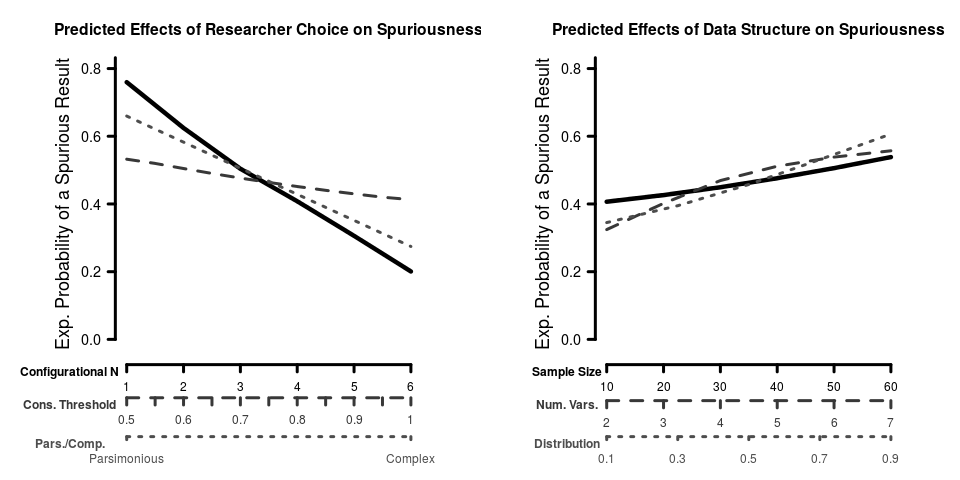
\includegraphics[scale=.7]{Plots/regression_plots.png}
	%\end{center}
\vskip-1ex
\caption{Relative Effects on the Probability of a Spurious Result in csQCA}
\end{sidewaysfigure}


\subsection{Results: The Differential Effect of Consistency Score Thresholds}

%This section probably needs more direct

Model 2 shows that the effect of consistency score threshold and configurational n threshold interacts strongly with the structure of the data. The effect of consistency score threshold on the odds of a spurious result is much greater when the distributions of all variables becomes less varied (i.e., when the marginal distribution of each variable is full of mostly 0s or 1s). Intuitively, as the variables contain more of just one value, the probability of a spurious result is much more affected by consistency threshold than when variables have a distribution closer to .5 (contains more of both 0s and 1s). The effect of consistency score threshold is also amplified when greater numbers of causal conditions are considered in a QCA model. 

Similarly, configurational n threshold has a greater effect at larger distributions. However, configurational n threshold has a slightly less pronounced effect when taking into account greater number of causal conditions. 


\subsection{Discussion: the Need for an Additional Robustness Assessment for QCA}

The section above showed that consistency score and configurational n thresholds have a differential effect upon spuriousness according to variations of basic features of the data. It is thus helpful to tune these thresholds, taking into account unique features of observed data. What would be useful, then, is a method that takes these features into account to give precise recommendations for researcher choices that provide robust results. The next section outlines a method that uses similar logic in providing these recommendations. 

\section{The Lieberson Robustness Assessment for QCA}

The Lieberson Robustness Assessment for QCA (LaQCA) is a procedural check of a QCA result that takes into account data structure (e.g. marginal distribution of variables) and researcher choice (e.g. consistency score threshold) to provide an estimate of the probability of spuriousness for a given QCA result. 

To do this, we draw several random data sets (like above), using the 1) same number of causal conditions as the observed QCA data set, 2) the marginal distributions of the causal conditions and dependent variable present in the QCA data, and 3) the sample size. We then run a QCA model matching 4) the consistency score threshold set by the researcher and 5) the configurational n threshold set by the researcher. After thousands of repetitions, we take the simple probability that QCA in this case returned a configuration. The inverse of this proportion can be interpreted as the confidence that the configuration returned in the real analysis is due to random chance. This interpretation is similar to the p-value used in regression analysis to determine the "significance" of a result. 

Convergence diagnostics, using r-hat values (ratio of variation within-simulation set to variation between simulation sets), were undertaken to determine how many simulations were needed to provide an accurate estimate, which determined about ~2000 simulations (). We also provide estimates of uncertainty using bootstrapped standard errors (). 

Below, we provide two case studies where a reasonable consistency score/configurational n threshold was sufficient to provide robust results, and a case where a robust result was not returned using these thresholds. 

\subsection{Qualitative Comparative Analysis of Tea Party Rallies in Florida}

%This is where a description of the data would be useful. 

To test our argument, we use a subset of data constructed by McVeigh and colleagues (2014) as part of their project on the emergence of Tea Party organizations in U.S. counties. The data set includes several county-level measures, including demographic measures from the American Community Survey (ACS) 2005-2009, measures of religious adherence from the Association of Religion Data Archives (ARDA) 2001, 2008 Presidential election measures from Congressional Quarterly's {\it{America Votes}}, and (although not included here) the number of Tea Party organizations between 2009 and 2010 from the Institute for Research and Education on Human Rights (IREHR). We extend the data set to include the a new outcome variable, the number of rallies in each county between 2009 and 2010, also from IREHR. 

We limit the data set to counties in Florida for two reasons. First, after winning the Senate seat in the 2010 midterm election, Marco Rubio credited his success to the help of the Tea Party movement and he has been dubbed (by some) as the crown prince of the movement (). Indeed, the Tea Party movement had a strong presence in Florida in 2010. Second, we choose Florida counties because, with the exception of California, all other states had fewer numbers of organizations. After limiting the data to the sample of Florida counties, we are left with 67 cases included in the analysis. Our analysis addresses the multiple causal pathways that lead to the occurrence of one or more Tea Party rallies in a Florida county.

\begin{figure}[htb!]
	\begin{center}
	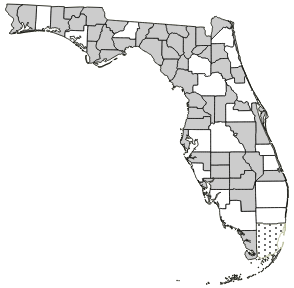
\includegraphics[scale=.75]{Plots/florida_rallies_cropped.png} %no spaces or it overlays the name of the file
	\end{center}
\caption{Tea Party Rallies in Florida Counties}
\label{diagram}
\end{figure}

Qualitative Comparative Analysis arguments are combinational and often overlapping, and a researcher's causal arguments often require a deep knowledge of cases in the data set for adequate placement within particular sets of causal arguments. For example, to fully belong to a crisp outcome set, a county must meet and/or exceed a minimum criterion. Therefore, it is necessary to both establish adequate causal argument and an inclusionary criteria for each causal argument. Lieberson () and others have argued that because these criteria are based on researcher selection, criteria are biased, essentially resulting in cherry-picked analyses. To combat this assumption, and for the sake of clarity, we employ a simple inclusionary-exclusionary criterion for membership in a variable set (outlined below) in the analysis. 

Research on the Tea Party movement has demonstrated that while most of their organizations were concentrated in conservative partisan environments (McVeigh et al. 2014, Skocpol and Williamson 2012), much of their on-the-ground rally and protest activity took place in heavily populated, left-leaning locales (Skocpol and Williamson 2012, Zernike 2010) (). For Tea Party organizations, research demonstrates the importance of educational background on support for the Tea Party (McVeigh et al. 2014, Skocpol and Williamson 2012), finding that supporters of the Tea Party movement are highly educated, and that Tea Party organizations were more likely to be established in U.S. counties characterized by a predominance of college graduates. Finally, although supporters of the Tea Party movement tended to be relatively shielded from the economic recession of 2008 (Skocpol and Williamson 2012, Parker and Barreto 2013), many of the movement's grievances consisted of dismay about unemployment, and how the federal government would expand it's reach, through a series of redistributive policies, to remedy the economic situation (Parker and Barreto 2013, McVeigh et al. 2014). 

The brief summary of research on the Tea Party, to date, provides insight into creating causal arguments about the presence of Tea Party rallies. Importantly, because the analysis here employs crisp-set Qualitative Comparative Analysis, each causal variable is coded as either one or zero. As previously mentioned, the outcome variable is Tea Party RALLIES. Full placement in the outcome set (1) requires that a county has at least one rally. Given the differential relationship between Republican partisan contexts and the presence organizations and the occurrence of rallies, I include a measure of REPUBLICAN. This is coded as one if, during the 2008 Presidential Election, the Republican candidate received a majority of the votes in the Florida county. Based on the above literature, I expect that the absence of (negation of) Republican context is an important component of a causal pathway to Tea Party rallies. I also include two variables where full inclusion is defined in a straightforward manner: full inclusion in the set is determined by whether or not a value for a particular case falls at or above the mean for that variable. First, I include a measure of COLLEGE educated, the percentage of people in the county (aged 25 or above) who hold a Bachelor's degree. Full membership in this set (1) is coded as whether or not the value for a county is equal to or above the mean value for college educated. Second, I included a measure of UNEMPLOYMENT, measured as the percent of the county population which is unemployed. If the case has a value at or above the mean unemployment rate for Florida, the county is given full membership in the set. With regard to membership in the college educated set, I expect that the presence of a college educated population is an important component of the pathway to rallies. However, given that many Tea Party supporters were not actually unemployed (although the movement's rhetoric says otherwise), I expect that the absence of a high unemployed population is an important part of explaining Tea Party rallies.

In QCA, the logical representation of the presence of a causal condition is indicated by the variable name in all capital letters whereas negation is represented by all lower case letters. Combinations of conditions (e.g. complex combinations of variables) in a pathway or recipe to an outcome are expressed as a string of variable names delineated by an asterisk, representing the logical operator "AND." If multiple pathways exist, each pathway is delineated by a plus symbol, the logical operator for "OR." Therefore, our main expectation, expressed in QCA notation, is:
\begin{center}
republican * COLLEGE * unemployment
\end{center}

In this analysis, there are a total of eight possible pathways to the outcome, based on the three ($K$) causal conditions ($2^K = 2^3 = 8$). The results in Table 1 indicated that only one combination (with 42.1\% coverage) explains the presence of Tea Party rallies in Florida counties. Overall, as expected, having a high college educated population, low levels of unemployment, and non-Republican partisan environments is critical for Tea Party rally occurrence. 

\begin{table}[h] %missing [] == [t], h is current position
\caption{QCA Results for Florida Tea Party Rallies} \label{tab:title} 
\begin{center}
\begin{tabular}{ >{$}l<{$}  >{$}c<{$} >{$}c<{$} >{$}c<{$}}
  \text{Solutions} &  & \text{Consistency} & \text{Coverage} \\
  \hline \hline
  & & & \\
  \text{republican * COLLEGE * unemployment} &  & 72.7\% & 42.1\% \\
  & & & \\
  \hline
\end{tabular}
\end{center}
\end{table}

\subsection{Application of the Lieberson Robustness Assessment}

% [Ben] is this where we run ltQCA, or the sim.ltQCA? Let me know. I can add more.

\subsection{Discussion} 

The two cases above show that identical thresholds of consistency and configurational n thresholds can vary greatly in terms of their robustness to randomness. If a researcher is concerned about a QCA result based strictly upon a possibility of spurious configurations, our case studies show that a consistency score/configurational n is not always effective in ensuring that a configuration is nonrandom. By taking into account truly random data, we show in the first case that a conventional consistency score is too conservative; in the second case, we show that a high consistency score is not quite enough to ensure robust configurations. Here, we more precisely estimate the probability of randomness via a direct comparison with random data."

%Figure A. Data distributions

%\section{Discussion}
%Something needs to be here...
%Using simulations, we showed that this can be assessed on a case-by-case basis. 

\section{Conclusion}

QCA can be robust to randomness using existing checks, but the ability of these checks to be able to sufficiently protect against spuriousness differs according to data structure. We present a method that measures the confidence that a given QCA result is due to random chance, which provides information above and beyond the current robustness checks. Ideally, the Lieberson Assessment could be used as a standard assessment for QCA that provides precise recommendations for researcher choice. 


\
\begin{center}
Works Cited
\end{center}

%\begin{hangparas}{.25in}{1}

%Adamic, Lada, And Natalie Glance. 2005. "The Political Blogosphere And The 2004 Us Election: Divided They Blog." \emph{Proceedings of the 3rd International Workshop On Link Discovery}.

%Gardner, Amy. 2010. ?Gauging the Scope of the Tea Party Movement in America.? Retrieved September 15, 2012 (http://www.washingtonpost.com/wp- dyn/content/article/2010/10/23/AR2010102304000.html?sid=ST2010110201489)

%McVeigh, Rory, Kraig Beyerlein, Burrel Vann Jr, And Priyamvada Trivedi. 2014. "Educational Segregation, Tea Party Organizations, and Battles Over Distributive Justice." \emph{American Sociological Review 79} 4: 630-652.

%Parker, Christopher S. and Matt A. Barreto. 2013. Change They Can?t Believe In: The Tea Party and Reactionary Politics in America. Princeton, NJ: Princeton University Press.

%Skocpol, Theda and Vanessa Williamson. 2012. \emphh{The Tea Party and the Remaking of Republican Conservatism}. Oxford University Press.

%Williamson, Vanessa, Theda Skocpol, and John Coggin. 2011. The Tea Party and the Remaking of Republican Conservatism. \emph{Perspectives on Politics 9} :25-43.

%Zernike, Kate. 2010a. \emph{Boiling Mad: Inside Tea Party America}. New York: Times Books.

 %\end{hangparas}


\end{document}